% !TEX TS-program = pdflatex
% !TEX encoding = UTF-8 Unicode


\documentclass[review, endfloat]{elsarticle}

\newcommand{\abbreviations}[1]{%
  \nonumnote{\textit{Abbreviations:\enspace}#1}}

\journal{Vaccine}

\usepackage[utf8]{inputenc}
\usepackage{graphicx}
\usepackage{booktabs}
\usepackage{hyperref}

\usepackage{soul}
\usepackage{xargs}
\usepackage[pdftex,dvipsnames]{xcolor}
\usepackage[colorinlistoftodos,prependcaption,textsize=tiny]{todonotes}
\newcommandx{\unsure}[2][1=]{\todo[linecolor=red,backgroundcolor=red!25,bordercolor=red,#1]{#2}}
\newcommandx{\change}[2][1=]{\todo[linecolor=blue,backgroundcolor=blue!25,bordercolor=blue,#1]{#2}}
\newcommandx{\info}[2][1=]{\todo[linecolor=OliveGreen,backgroundcolor=OliveGreen!25,bordercolor=OliveGreen,#1]{#2}}
\newcommandx{\improvement}[2][1=]{\todo[linecolor=Plum,backgroundcolor=Plum!25,bordercolor=Plum,#1]{#2}}

\title{Surveillance for adverse events following live attenuated herpes zoster vaccine: a self-controlled case series analysis using general practice data}

% Authors and affiliations

\author[1]{James Totterdell\corref{cor1}}
\ead{jamestotterdell@telethonkids.org.au}
\author[2]{Anastasia Phillips}
\author[3]{Catherine Glover}
\author[1]{Julie Marsh}
\author[3]{Kristine Mccartney}
\author[1]{Tom Snelling}
\author[4]{Kendall Chidwick}

\cortext[cor1]{Corresponding author}
\address[1]{Wesfarmers Centre for Vaccines and Infectious Diseases, Telethon Kids Institute}
\address[2]{University of Sydney}
\address[3]{National Centre for Immunisation Research and Surveillance}
\address[4]{NPS MedicineWise}

\begin{document}

\begin{frontmatter}

\begin{abstract}

\emph{Objective}: To investigate the risk of pre-specified adverse events following live attenuated herpes zoster vaccine (ZVL) in older adults attending primary care providers in Australia.

\emph{Methods}: Individuals aged 70 to 79 years who received ZVL between 1 November 2016 and 31 July 2018 were identified within a nationally representative primary care database. The self-controlled case series (SCCS) method was used to estimate the seasonally-adjusted relative incidence (RI) of seven outcome events (injection site reaction (ISR), burn [negative control], myocardial infarction (MI), stroke, any rash, rash with a prescription for an antiviral within 2 days of the rash-related encounter, and clinical attendance) during a post-vaccination, at-risk window compared with a time distant to vaccination. Sensitivity analyses examined the effect of concomitant vaccination (influenza and 23-valent pneumococcal vaccination) and restriction to first outcome event. 

\emph{Results}: A total of 332,988 vaccination encounters in 150,054 individuals were identified during the study period. The most common outcome identified was clinical attendance (\textgreater 2 million events) followed by rash (12,309 events); ISR was the rarest outcome (177 events). There was an increased RI of ISR in the 7 days following ZVL (RI = 77.4; 95\% CI = [48.1, 124.6]). No increase to the RI of MI (0.74; [0.41, 1.33]), rash (0.97; [0.8 to 1.08]), or rash with antiviral (0.83; [0.62 to 1.10]) were evident in the 42 days following ZVL. The RI of clinical attendance (0.94; [0.94, 0.95]) and stroke (0.58; [0.44, 0.78]) were lower in the 42 days following administration of ZVL.

\emph{Conclusions}: No new safety concerns were identified for ZVL in this study based on a novel primary care data source using an SCCS design. An expected increased risk of ISR was identified; findings in relation to cardiovascular disease were reassuring.

\end{abstract}

\begin{keyword}
zoster vaccine \sep self-controlled case series \sep surveillance \sep vaccine safety
\end{keyword}

\abbreviations{CI, confidence interval; ISR, injection site reaction; MI, myocardial infarction; RI, relative incidence1; SCCS, self-controlled case series; ZVL, live attenuated herpes zoster vaccine.}

\end{frontmatter}


\section{Introduction}

Herpes zoster (HZ) is a localised, painful, vesicular skin rash resulting from reactivation of varicella-zoster virus. The average lifetime risk is around 30\% but increases with age \citep{brisson2001epidemiology}. Prior to implementation of vaccination programs, the incidence of HZ in Australia was reported to be 10 per 1000 persons aged 50 years and older \citep{stein2009herpes}, similar to rates observed in Europe \citep{pinchinat2013similar} and the United States (US) \citep{insinga2005incidence}. The risk of post-herpetic neuralgia, a chronic neuropathic pain syndrome commonly following HZ, also increases with age. Disseminated disease can occur in people who are immunosuppressed. 

Live attenuated varicella-zoster vaccine (ZVL) was registered for use in Australia in 2006 and available from 2014 for people aged over 50 years \citep{yawn2007population}. It is recommended for immunocompetent adults over 60 years of age. In November 2016, a funded ZVL immunisation program commenced under the Australian National Immunisation Program (NIP) for adults aged 70 years, with catch-up for those aged 71–79 years funded until October 2021. 

ZVL was evaluated in large, pre-licensure clinical trials with no increased risk of serious adverse events (SAE), hospitalized adverse events or death \cite{oxman2005, gagliardi2016vaccines, schmader2012}. The rate of injection site reactions (ISR) was higher in vaccine than placebo groups \cite{oxman2005, schmader2012}. A post-licensure clinical trial demonstrated a similar safety profile, with no statistically significant difference in the rate of SAE up to 182 days following vaccination \citep{murray2011}. Post-licensure passive surveillance has been consistent with clinical trials. Of 23,556 reports submitted by healthcare providers to the Merck, Sharp, \& Dohme Corp (MSD) Adverse Event (AE) global safety database between May 2006 and May 2016, 93\% of reports were non-serious, with ISR the most commonly reported AE (20.5\%), followed by HZ (8.6\%) and rash (4.2\%) \citep{willis2017herpes}. Of 23,092 reports submitted to the US Vaccine Adverse Events Monitoring System (VAERS) from May 2006 to January 2015, 96\% were classified as non-serious, with ISR, HZ and rash the most frequently reported non-serious AE \citep{miller2018post}.

In Australia, AusVaxSafety is an active vaccine safety surveillance system that monitors adverse events following immunisation using data reported directly from people receiving the vaccines (or their parent or carer) with responses solicited via an automated SMS or email. Active surveillance of zoster vaccine safety conducted from 1 November 2016 to 4 November 2018 identified no safety signals amongst 18,655 adults aged 70-79 years where 8.3\% of vaccinated individuals reported an adverse event \citep{ausvaxsafety}.

Post-marketing surveillance methods are limited by the potential for biased reporting and, for ZVL, is confounded by the higher prevalence of chronic disease in the older target population \citep{miller2018post}. The self-controlled case series (SCCS) method was developed for vaccine safety assessment and has the potential to automatically adjust for unmeasured time-invariant confounders by allowing individuals to act as their own control \citep{petersen2016}. SCCS methodology has previously been used to examine ZVL using US data from managed care cohorts \citep{tseng2012} and administrative claims data \citep{minassian2015}. In Australia, older patients typically receive ZVL from their general practitioner (GP). While practices maintain their own electronic patient records, the Australian Government Department of Health funds NPS MedicineWise to collate GP data through the MedicineInsight program. 

The objective of this study was to use nationally representative GP data from MedicineInsight to examine the risk of pre-specified AE following ZVL in the target NIP cohort.

\section{Methods}

\subsection{Study setting}

The MedicineInsight data set consists of longitudinal, de-identified, whole-of-practice data extracted from the clinical information systems (CIS) of participating general practice sites across Australia. These include sites in major cities and in rural and remote areas, similar to the distribution of the Australian population over these areas. The participating sites represent between 15\% and 20\% of the Australian population.  Data is extracted on patient demographics, practice encounters (excluding progress notes), diagnoses, vaccinations, prescriptions, pathology tests and referrals. Practice encounters can include clinical (a medical or nursing appointment) or non-clinical (an entry by administration staff) encounters. Within-site individual identifiers are used to identify records common to an individual attending that site. \improvement{Citation for representativeness of MedicineInsight? Databook/website/GP insights reports?}

\improvement{Perhaps discuss how clinical information is recorded e.g. the Docle and PyFinch systems. Input manually by practice staff.}

\subsection{Study population}

The target population was individuals aged 70-79 years who were eligible to receive ZVL, 23-valent pneumococcal (23vPPV), or seasonal inactivated influenza vaccine. Although the primary vaccine of interest was ZVL, individuals who had received 23vPPV and seasonal inactivated influenza vaccines were also included for two reasons: ZVL may commonly be co-administered with these two vaccines meaning that any events identified might be attributable to these other vaccines; and to estimate the relative incidence of adverse events in other vaccines using the same data source and methods as a comparator for the ZVL estimates.  All MedicineInsight records were obtained for individuals 70–79 years of age at the date of their vaccination who received ZVL, 23vPPV or influenza vaccine(s) between 1 November 2016 (when the funded ZVL program began) to 31 July 2018. We treated this study population as a random sample of the target population. 

Individuals with a history of stroke and myocardial infarction were identified by a search of their site history for practice encounters and diagnoses related to these conditions. Individuals with records for historical events of stroke and myocardial infarction (those occuring before the start of the study period) were excluded . Individuals who died were censored at 31 December of the preceding year because only the year of death was available. 

\subsection{Study design}

We undertook a retrospective SCCS analysis of adverse events following ZVL using MedicineInsight data. The SCCS design was developed for vaccine safety evaluation \citep{farrington1995} and has been used in a variety of settings \citep{buttery2011intussusception, bakken2015febrile, stowe2016risk}. The method estimates the relative incidence of an outcome event within a risk window following exposure (i.e. vaccination) compared to the incidence at all other times under observation. Only individuals who have experienced an outcome event contribute to the relative incidence estimate and the design potentially controls for time-invariant confounders.

This study investigated the relative incidence of seven pre-specified outcome events (ISR [positive control], burn [negative control], myocardial infarction, stroke, any rash, rash with a prescription for an antiviral within 2 days of the rash-related encounter, and clinical attendance) in a post-vaccination, at-risk window, with the incidence of these outcome events at times distant from vaccination. ISR was included as a positive control given consistent evidence of an increased risk of ISR in pre-licensure and post-licensure studies. Burn was included as a negative control with any events considered unrelated to vaccination.  

Events for individuals in the study population may not have been observable throughout the entirety of the study period. We defined an individual’s observation period in terms of their historical activity at the site and year of death information. An individual’s start date of observation was defined as the latest of 1 November 2016, or 365 days after their first recorded activity at the site (any encounter, diagnosis, or prescription record). An individual’s end date of observation was defined as 31 December in the year prior to their death for individuals who had year of death recorded, and 31 July 2018 for individuals who had no year of death recorded. The lead time of 365 days from an individual’s start of site activity was specified to allow for a catch up in medical information. The maximum possible observation period for any individual was 638 days.

Exposure (vaccination) was defined as an immunisation record for any of the three vaccines under study with a date of administration occurring within the individual’s observation period. Due to the mix of clinically coded and free text entries, vaccination records for the study vaccines were identified via targeted, free-text search criteria. The date of vaccination was set as the administration date specified in the vaccination record. Individuals with multiple vaccination records for ZVL or 23vPPV during their observation period were excluded as these vaccines are generally recommended to be given as a single dose for older adults. We enforced a minimum time between influenza vaccinations of 126 days because a single dose is generally recommended each season. Any influenza records occurring within 126 days of an individual’s previous influenza vaccintation were excluded from analyses to avoid overlapping risk-windows (\autoref{sec:risk_windows}). Any vaccines with the same recorded date of administration were assumed to be co-administered.

Except for clinical attendance, outcome events were identified using free-text regular expression searches of reason for encounter, reason for diagnosis and reason for prescription fields. For each record matching an outcome event, we matched encounters, diagnoses, and prescriptions on their respective dates to combine related events and then ordered all records by date of occurrence. 

Records of clinical attendance were defined as any site encounter record excluding those identified to be non-clinical (administrative). Non-clinical records were identified and excluded by a free-text search of the encounter type and encounter reason field for specific terms identified as administrative in nature. 

Individuals were defined as cases with respect to an outcome if they experienced at least one event for that outcome during their observation period.

\subsection{Definition of risk windows}
\label{sec:risk_windows}

At-risk windows were defined consistently for all vaccine types based on biologically plausible windows supported by evidence. For ISR the risk-window was 1–7 days post vaccination, and for all other outcomes was 1–42 days post vaccination. The basis for the length of the risk window for systemic adverse events was the 42 day window used in pre-licensure clinical trials \citep{oxman2005, schmader2012, murray2011, simberkoff2010} and post-licensure studies \citep{tseng2012,baxter2012}. This time period is also biologically plausible for cardiovascular events, which have been observed following wild-type varicella-zoster virus, particularly 1 to 4 weeks following infection \citep{minassian2015,schink2016}, with viral replication in arterial walls the proposed mechanism for cerebrovascular disease \citep{gilden2009}. This risk window is also biologically plausible for rash, with varicella-like rash after 6 weeks more likely to represent wild-type infection \citep{willis2017herpes}. The risk windows for burn (the negative control) and clinical attendance were chosen to be consistent with the risk window for systemic events. For ISR, the risk window was based on the short median time to ISR (\~2 days) in the Shingles Prevention Study (SPS) and post-licensure surveillance \citep{willis2017herpes,simberkoff2010} and the identification of a signal for cellulitis within 7 days in another post-licensure SCCS \citep{tseng2012}.

To account for the potential for an event to affect the likelihood of vaccination a pre-exposure washout period of 42 days pre-vaccination was defined for all outcomes. A 42 day post-risk washout period was also included to minimise the potential for risk that may be attributable to the vaccine to carry over into the control period. For rash with antiviral, an indefinite post-risk period was specified due to an expected reduced risk following ZVL vaccination. In allowing an indefinite risk period following influenza, overlapping risk periods may be encountered, and therefore for this outcome only the first recorded influenza vaccination was considered for analysis.

Pre-exposure and post-risk washout periods were excluded from the control period. The day of vaccination was excluded from all analyses. This was due to individuals having numerous encounters or diagnoses coinciding with the vaccination encounter. We assumed such encounters to be unrelated to the vaccine administered during that encounter. All other time an individual was under observation was allocated to their control period.

\begin{figure}
\caption{Self-controlled case series study design.}
\label{fig:sccs_design}
\end{figure}

\subsection{Statistical methods}
\label{sec:stat_methods}

Relative incidence estimates were obtained from an SCCS model \citep{farrington2018} using the windows previously defined. Given that the study period spanned 1 November 2016 to 31 July 2018, we additionally specified fixed windows to adjust for seasonal effects by specifying window cut-points: 1 December, 1 March, 1 June, and 1 September in each year. Each outcome was modelled independently. The main analyses modelled all exposures (vaccines) jointly assuming additive effects in overlapping risk-windows and allowed for recurrent events for each outcome with all outcome events occurring during the observation period contributing towards the relative incidence estimate. Weekly periodicity of events was accounted for indirectly by the specification of risk-windows in terms of full-week cycles.

Dependence of outcome events violates the Poisson assumption of the SCCS model and may bias estimates. Recurrent event dependencies were explored visually by looking at Nelson-Aalen estimators for the cumulative hazard and histograms of gap times. Sensitivity analyses were undertaken which only included the first outcome event observed.  Sensitivity analyses assessing each vaccine independently, excluding co-administered vaccines from the analysis, were also undertaken. 

The relative incidence and 95\% CIs for each outcome were estimated using Poisson regression with length of windows included as offset terms. No adjustments were made for multiple comparisons. All analyses were conducted using R 3.5.1 \citep{rmanual} and the gnm package version 1.1-0 \citep{rgnm}.

\subsection{Ethical approval}

This MedicineInsight program was approved through the Royal Australian College of General Practitioners National Research and Evaluation Ethics Committee (NREEC) in December 2017 (NREEC 17-017). Approval for use of MedicineInsight data in this study was received from the NPS MedicineWise external Data Governance Committee on 23 November 2016 and an amended version on 29 September 2017.This study was also approved by the Sydney Children’s Hospitals Network Human Research Ethics Committee (HREC/17/SCHN/159). 

\section{Results}

\subsection{Vaccinations and outcome events}

A total of 337,294 vaccination records for 150,756 individuals from 456 MedicineInsight sites were identified. After excluding individuals with multiple ZVL or 23vPPV vaccinations, and excluding multiple influenza vaccinations occurring within 126 days of each other, a total of 332,988 vaccinations (ZVL: 92,857, 23vPPV: 21,480, and influenza: 218,651) for 150,054 individuals remained for inclusion in the analysis. According to our criteria, the majority of individuals (93\%) were deemed to be under observation for the entire study period.

ZVL vaccinations occurred more commonly at the beginning of the study period following its addition to the NIP. Expected weekly cycles and seasonal fluctuations in vaccination counts were observed amongst the three vaccines investigated (\autoref{fig:vax_dates}). In general, the number of vaccination records declined with age with ZVL increasing slightly at 79 years of age (\autoref{fig:vax_ages}). ZVL was commonly co-administered with influenza vaccine (16\% of ZVL vaccinations) and sometimes with 23vPPV (2\% of ZVL vaccinations). 23vPPV and influenza vaccine were often co-administered (43\% of 23vPPV vaccinations).

Over 2 million clinical attendances were observed among exposed individuals during their observation periods. The most common outcome event was any rash, with 12,309 events observed. The rarest outcome event was injection site reaction, with 177 events observed.

\begin{figure}
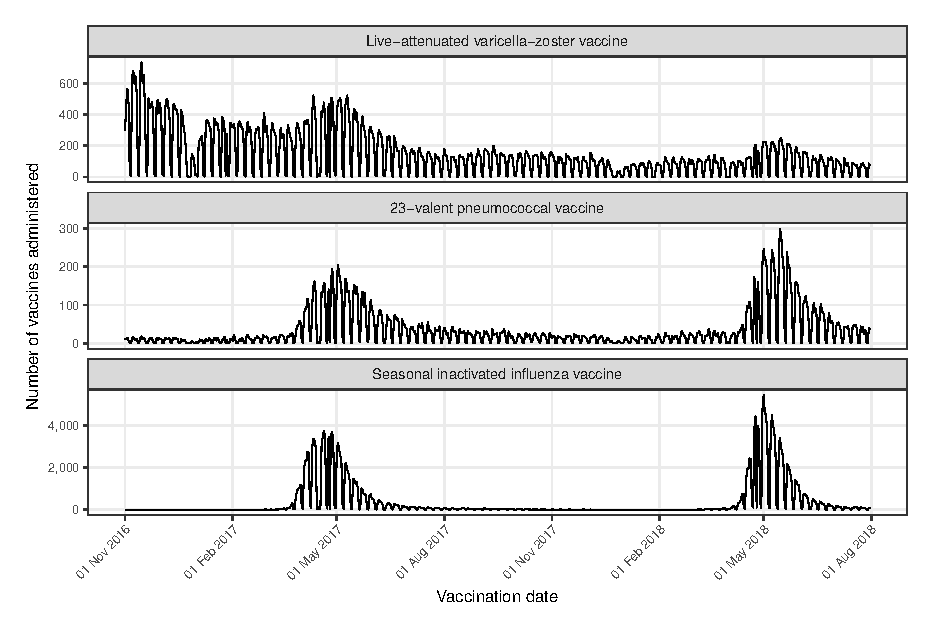
\includegraphics{figs/exposure_time_series}
\caption{Daily counts of vaccinations administered during the study period.}
\label{fig:vax_dates}
\end{figure}

\begin{figure}
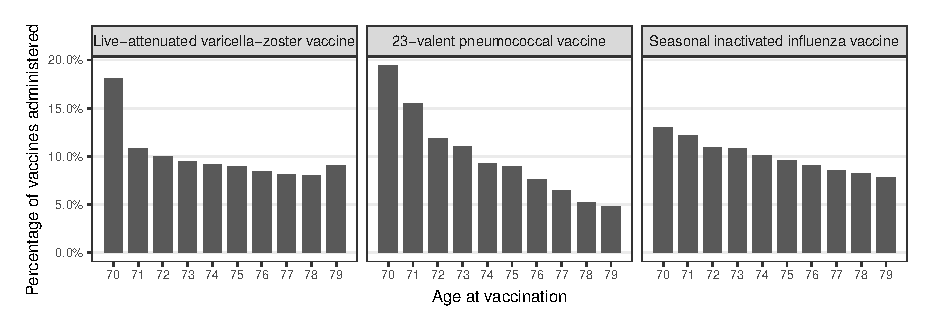
\includegraphics{figs/age_at_exposure}
\caption{Distribution of age at vaccination.}
\label{fig:vax_ages}
\end{figure}


\subsection{Self-controlled case series analysis}

\begin{table}
	\centering
	\caption{Relative incidence in at-risk period versus control period of all outcomes (modelled independently) for all vaccines, adjusted for season.}
	\label{tab:ri}
	\resizebox{\textwidth}{!}{%
	\begin{tabular}{lrrrrrrrrr}
		\toprule
		& \multicolumn{3}{c}{Zoster vaccine} & \multicolumn{3}{c}{Pneumococcal vaccine} & \multicolumn{3}{c}{Influenza vaccine}\\
		\cmidrule(lr){2-4} \cmidrule(lr){5-7} \cmidrule(lr){8-10}
		& At-risk & Control & & At-risk & Control & & At-risk & Control & \\
		& n (PD) & n (PD) & RI (95\% CI) & n (PD) & n (PD) & RI (95\% CI) & n (PD) & n (PD) & RI (95\% CI)\\
		\midrule 
		Injection site reaction & 37 (833) & 104 (96 876) & 77.4 (48.1, 124.6) & 30 (378) & 138 (102,318) & 65.0 (31.6, 133.6) & 29 (1,071) & 102 (84,934) & 6.62 (3.42, 12.8) \\
		
		Burn & 72 (23,798) & 1,282 (511,166) & 1.23 (0.97, 1.57) & 8 (5,259) & 1,455 (564,087) & 0.55 (0.27, 1.13) & 145 (57,946) & 1,036 (407,960)&0.93 (0.76, 1.14)\\
		
		Myocardial infarction & 12 (8,327) & 436 (221,244) & 0.74 (0.41, 1.33) & 2 (2,729) & 469 (237,376) & 0.39 (0.09,1.59) & 47 (23,226) & 324 (176,808) & 1.17 (0.82, 1.66) \\
		
		Stroke & 50 (35,113) & 1,984 (793,445) & 0.58 (0.44, 0.78) & 15 (9,081)& 2,132 (868,410) & 0.72 (0.42, 1.21) & 197 (88,397) & 1,500 (633,321) & 1.06 (0.89, 1.26)\\
		
		Any rash & 422 (228,311)& 10,381 (4,990,170) & 0.97 (0.88, 1.08) & 115 (52,961) & 11,959 (5,497,005) & 1.01 (0.84, 1.23) & 1,124 (564,634) & 8,645 (3,982,480)& 1.06 (0.98, 1.14) \\
		 
		Rash with antiviral & 61 (33,800) & 1,570 (856,854) & 0.83 (0.62, 1.10) & 22 (10,571) & 1,931 (1,099,845) & 1.23 (0.77, 1.95) & 104 (73,998) & 917 (455,454) & 0.78 (0.62, 0.97) \\
		
		Clinical attendance & 79,352 (3,726,764)& 1,799,288 (79,138,828)& 0.94 (0.94, 0.95)& 19,616 (848,864)& 2,032,393 (87,483,370)& 1.06 (1.04, 1.07)& 200,785 (8,840,389)& 1,368,928 (63,862,675) & 1.03 (1.02, 1.03)\\
		
		\bottomrule
		\multicolumn{10}{l}{RI: relative incidence of at-risk compared to control, PD: person-days.}
	\end{tabular}}
\end{table}

\begin{table}
	\centering
	\caption{Sensitivity analyses: relative incidence in at-risk period versus control period of all outcomes for Zostavax with and without concomitant vaccines and considering all events or first events only.}
	\label{tab:ri_sens}
	\resizebox{\textwidth}{!}{%
	\begin{tabular}{lrrrr}
		\toprule
		& \begin{tabular}{@{}c@{}}Vaccines modelled jointly \\ all events \end{tabular} & 
		\begin{tabular}{@{}c@{}}Vaccines modelled independently \\ (concomitant vaccines excluded) \\ all events \end{tabular} & 
		\begin{tabular}{@{}c@{}} Vaccines modelled jointly \\ first events only \end{tabular} & 				\begin{tabular}{@{}c@{}} Vaccines modelled independently\\ (concomitant vaccines excluded)  \\ first events only \end{tabular} \\
		\midrule 
		Injection site reaction & 77.4 (48.1, 124.6) & 60.5 (37.4, 97.9) & 71.2 (43.6, 116.1) & 57.3 (34.8, 94.3) \\
		Burn & 1.23 (0.97, 1.57) & 1.12 (0.86, 1.47) & 1.08 (0.78, 1.50) & 1.12 (0.80, 1.58) \\
		Myocardial infarction & 0.74 (0.41, 1.33) & 0.70 (0.35, 1.36) & 0.90 (0.49, 1.66) & 0.80 (0.39, 1.64) \\
		Stroke &0.58 (0.44, 0.78)& 0.51 (0.37, 0.71)& 0.54 (0.37, 0.77)& 0.51 (0.34, 0.76) \\
		Any rash & 0.97 (0.88, 1.08) & 0.96 (0.86, 1.07) & 1.01 (0.90, 1.14) & 1.01 (0.89, 1.14) \\
		Rash with antiviral & 0. 83 (0.62, 1.10) & 0.67 (0.49, 0.92) & 0.80 (0.59, 1.09)& 0.64 (0.45, 0.90)\\
		Clinical attendance & 1.23 (0.97, 1.57) & 0.94 (0.93, 0.94) & NA & NA \\
		\bottomrule
	\end{tabular}}
\end{table}

\subsubsection{Injection site reactions}

An increase in the relative incidence of injection site reactions was observed in the 7-day risk window following all three vaccines in the main analysis (\autoref{tab:ri}). This was consistent in sensitivity analyses excluding co-administered vaccines (\autoref{tab:ri_sens}).

In all analyses, the incidence of ISR remained elevated in the 42-day post-risk period following ZVL (RI = 3.4, 95\% CI [1.8, 6.5] based on main analysis). A 7-day partition of this period identified that incidence remained elevated 8 to 14 days post-vaccination (RI = 16.2, 95\% CI [6.8, 38.7]) before returning to control period levels.

\subsubsection{Myocardial infarction}

There was no increased risk of myocardial infarction following any vaccine in the main analysis (\autoref{tab:ri}) or when including first events only as part of a sensitivity analysis (Table 3). 

An increased relative incidence was observed during the post-risk washout period (days 43–84) for ZVL in the main analysis (RI = 1.7, 95\%CI [1.1, 2.5]). The increased relative incidence of MI in the post-risk washout period following ZVL was also observed in sensitivity analyses for first events only (RI = 1.8, [1.2, 2.8]) and first events excluding co-administered vaccines (RI = 2.1, [1.3, 3.4]) (\autoref{tab:ri_sens}).

\subsubsection{Stroke}

In the main analysis, a reduced relative incidence of stroke was observed following ZVL. This effect continued into the post-risk washout window (RI = 0.7, 95\% CI [0.5, 0.9]). In a sensitivity analysis considering only first stroke events, the incidence was reduced only during the at-risk period.

\subsubsection{Rash}

There was minimal change in the risk of rash or rash with antiviral  following ZVL compared to the control period in the main analysis (Table 2), although a reduced risk was apparent in the post-risk washout period (RI = 0.67, 95\% CI [0.54, 0.83]) for rash with antiviral. There was a reduced risk for rash with antiviral following ZVL in the sensitivity analysis where co-administered vaccines were excluded (Table 3).

\subsubsection{Clinical Attendance}

There was a small reduced incidence of clinical attendance following ZVL and a small increased incidence of clinical attendance following 23vPPV and influenza vaccines (\autoref{tab:ri}). These associations held in the sensitivity analysis for individual vaccines ZVL and 23vPPV, but there was no increased risk for clinical attendance following influenza vaccination given alone.

\subsubsection{Burn}

No change in the incidence of burn, which was used as a negative control, was observed for any of the vaccines.

\section{Discussion}

The results of this SCCS analysis of MedicineInsight GP data provide evidence to support the safety of ZVL in individuals aged 70–79 years. An expected increased incidence of ISR up to at least 7 days following vaccination was observed following all three vaccines. In the SPS safety sub study, ISR were more common in vaccine (48\%) compared to placebo (16\%) recipients \citep{simberkoff2010}. The intensity of erythema and swelling were significantly greater in vaccine recipients and persisted for longer, although fewer than 1\% of vaccine recipients reported them as severe. A post-marketing study of 193,083 adults aged over 50 years in eight US managed care organisations demonstrated a small but significant increased risk of cellulitis and infection one to seven days following vaccination using the case-centred method \citep{tseng2012}. In our study, we observed elevated incidence if ISR up to 14 days following ZVL. While the SPS sub study did demonstrate ISR significantly later in vaccine recipients compared to placebo recipients, events still occurred a median of 2.3 days following vaccination. Similarly, in global passive surveillance, ISR have been reported at a median of 2 days following vaccination \citep{willis2017herpes}. In this SCCS, the risk of ISR was also elevated in the sensitivity analysis that excluded concomitantly administered vaccines. Similarly, a clinical trial of ZVL administered concomitantly with influenza vaccine, ISR and systemic reactions were comparable in those administered the vaccines concomitantly versus ZVL alone \citep{levin2018immunogenicity}.

It was reassuring that ZVL was associated with a reduced risk of clinical attendance following vaccination. This is consistent with pre-licensure studies which found no increased risk of serious adverse events \citep{oxman2005, gagliardi2016vaccines, schmader2012}. Similarly, it was reassuring that there was no increased risk of MI or stroke identified following ZVL. Although there is a reported risk of ischemic  and haemorrhagic stroke and myocardial infarction \citep{minassian2015, schink2016} in the 1 to 4 weeks folowing infection with wild-type herpes zoster virus \citep{gilden2009}, the SPS did not identify an increased risk for cardiovascular events. Post-licensure studies have not identified an increased risk for inpatient or ED encounters with cardiovascular or cerebrovascular events \citep{tseng2012}, and no temporal clustering of events following vaccination with ZVL has been observed \citep{baxter2012}.

VAERS post-marketing passive surveillance identified 3 deaths due to stroke and 28 due to heart disease in ZVL-vaccinated individuals between May 2006 and January 2015. The authors noted that some deaths from heart disease and stroke following ZVL would be expected in this age group due to chance alone. No unusual pattern was observed that would suggest a causal relationship to ZVL \citep{miller2018post}. The SCCS methodology used in this study supports the safety of ZVL with a reduction in the confounding that may affect passive surveillance systems. We note an observed higher relative incidence for MI our specified post-risk washout period (between 43 and 84 days following vaccination). Within this washout period, there was no consistent pattern of increased risk, with higher relative incidence on days 57 to 63 and 71 to 77, but not earlier (43 to 56 or 64 to 70 days). Whether this increased risk several months after vaccination relates to age-related confounding or other potential biases within the data requires further investigation. 

Similarly, estimated reduced risk of stroke following ZVL in this SCCS may be biased by the use of general practice (rather than hospital) data. Further investigation within emergency department and hospital data may provide greater sensitivity in identifying and validating cardiovascular outcome events. However, while presentation of cardiovascular and cerebrovascular events may be limited in the general practice setting, rash is a common presentation to general practice \citep{ely2010}. While rash has been considered a non-specific finding in post-marketing observational studies \citep{tseng2012}, the pairing of rash with antiviral prescription is likely to represent a more specific outcome event. A reduced risk of rash with antiviral following ZVL was identified, which may suggest vaccine efficacy or be considered reassuring given that a herpes zoseter-like rash may be a marker of disseminated infection if a patient is immunocompromised \citep{alexander2018}. In a recent survey of immunisation providers in the US, family physicians report recommending ZVL to immunocompromised populations, even though being immunocompromised is a contraindication to ZVL vaccination \citep{hurley2018}. In Australia in 2016, a death was reported following administration of ZVL to an immunocompromised individual who developed a vesicular facial rash 22 days after receiving ZVL, followed by disseminated infection and meningoencephalitis\citep{alexander2018}. This event led to widespread dissemination of education to GPs regarding appropriate administration of ZVL \citep{tgazos}.

Recently, the US Advisory Committee on Immunization Practices (ACIP) has recommended the new non-live recombinant herpes zoster subunit vaccine be used in preference to ZVL for in immunocompetent adults aged 50 years and older \citep{dooling2018}. The new vaccine was registered in Australia in July 2018 and while efficacy has been demonstrated, and it is not contraindicated in immunocompromised individuals \citep{hurley2018}, a recent meta-analysis suggests that it may be associated with more ISR than ZVL \citep{tricco2018}.

Although our results are reassuring, there are limitations to the use of MedicineInsight data and the methods which were applied. An key requirement of the analysis is that if an event occurred during an individuals' observation period it would have been ascertained. However, the quality of data used is dependent on GP data entry into the on-site clinical information system. Where an outcome was not recorded, it is not possible to know whether this reflected an absence of the outcome or of documentation, particularly for minor outcomes such as ISR. As not all data were coded, exposures and outcome events were identified by regular expression searches of text strings, which were not validated. Additionally, individual identifiers were only available at the site level, meaning any individuals attending multiple sites were treated as distinct individuals at each site. This meant that oucome events occurring at a site other than the one attended for vaccination would not be ascertained. However, evidence suggests multiple practice attendance may be lower in the older age groups we investigated \citep{wright2018}. Outcomes such as stroke and MI may be more likely to present to an emergency department than to primary care, such that general practice data may be insufficiently sensitive to monitor these events. 

It was not possible to determine exact event onset dates as these could only be inferred from the encounter, diagnosis, or prescription date recorded. The SCCS method requires precise information on the timing of the exposure and outcome events, and for the outcome events we considered, the date of condition onset is important. The reliability of using site attendance or diagnosis date as a proxy for condition onset is unknown. The relationship between dates recorded in the CIS and the timing of the event itself likely varies by site and practitioner. It was also not possible to determine an individuals level of immunocompetency due to the complexity of classifying the immune status of individual patients based on limited information; immune status may affect the experience of adverse events \citep{alexander2018, greenbook}. 

The use of general practice data and the SCCS design is a critical step in moving beyond passive surveillance and its inherent limitations. In Australia, many patients, especially older patients, see a regular general practitioner and GPs are immunisation providers for most patient cohorts. There is significant scope to better utilise routinely collected GP data for vaccine safety surveillance once the limitations and applications are more fully understood and validation of methodology has occurred. Linkage with hospitalisation data in Australia will make primary care data a rich source of information.

\section{Conclusion}

No new safety concerns were identified for ZVL in this study based on a novel data source using an SCCS design. Expected findings in relation to the positive (ISR) and negative (burn) control conditions support the validity of the SCCS analysis in this setting using general practice data. Findings in relation to cardiovascular disease and stroke were reassuring. Further work should focus on validation of identified exposures and outcomes and linkage with hospitalisation data and within sites.

\section{Disclaimer}

\section{Declaration of interest}

\section{Acknowledgements}

\section{Funding/Support}

\listoftodos[Notes]


\bibliographystyle{elsarticle-num-names}
\bibliography{ausvax-paper}

\end{document}
